\chapter{Evaluaci\'on de rankings sobre benchmarks}
\label{sec:evaluacion}

En este cap\'itulo se presentan diversas formas de evaluar a los algoritmos propuestos en el cap\'itulo anterior. En particular, se muestra que el algoritmo de refinamiento probabil\'{i}stico con sobreespecificaci\'on es capaz de generar un ranking de ERs que es similar a la distribuci\'on de frecuencias de las ERs observadas en corpora usando m\'etricas autom\'aticas y que tambi\'en tiene un buen desempe\~no cuando se usan m\'etricas manuales. Parte de esta evaluaci\'on fue presentada en el paper \cite{context2013}. 

Este cap\'itulo est\'a dividido en 4 secciones, en la Secci\'on \ref{sec:compara} se muestra una evaluaci\'on autom\'atica con respecto al GRE3D7. En la Secci\'on \ref{sec:automaticevaluation} se presenta una evaluaci\'on autom\'atica con respecto a resultados de una competencia sobre el corpus TUNA. Luego en la Secci\'on \ref{sec:humanevaluation} se presenta una evaluaci\'on de jueces humanos con respecto al corpus TUNA. Para finalizar en la Secci\'on \ref{sec:notas5} se describe el resumen y linkeo del cap\'itulo.

\section{Evaluaci\'on de rankings sobre el corpus GRE3D7}
\label{sec:compara}
En esta secci\'on presentamos una evaluaci\'on cuantitativa y autom\'atica de los algoritmos en el dominio del corpus GRE3D7~\cite{gre3d7} introducido en la Secci\'on~\ref{sec:corpusGRE} del Cap\'itulo~\ref{sec:seleccion}. Mostraremos una comparaci\'on con el ranking de ERs dadas por el algoritmo con las probabilidades de uso calculadas como se describe en la Secci\'on~\ref{sec:learning}, es decir con aprendizaje autom\'atico a partir de las dem\'as im\'agenes del corpus y ejecutando nuestro algoritmo 10000 veces. El algoritmo probabil\'istico con sobreespecificaci\'on es capaz de generar una distribuci\'on de ERs similar a la que se observa en el corpus. Describimos primero en detalle los experimentos que realizamos para la escena que se muestra en la Figura~\ref{contexto-evaluacion}, en la Secci\'on \ref{sec:caso_estudio_gre3d7}. Luego, en la Secci\'on \ref{sec:compara-varias}, resumimos los resultados obtenidos en evaluaciones similares para otras 7 escenas del corpus. 
\subsection{Caso de estudio de una escena del corpus}
\label{sec:caso_estudio_gre3d7}
Las probabilidades de uso aprendidas usando regresi\'on lineal como se muestra en la Secci\'on~\ref{sec:learning} se muestran en la Tabla \ref{probabilidades-escena2}.

\begin{table}[h]
\begin{center}
\footnotesize{
\begin{tabular} {  l c c c c c c c c c c c}
\hline
R				&{\it ball}			& {\it cube}	& {\it green}	  & {\it blue} & {\it large} & {\it small} & {\it ontop}& {\it left}  & {\it top} & {\it front}   &{\it below} \\
\hline
R.\puse	& 1.0			& 1.0		& 0.993& 0.124&0.03  &0.346   &0.179 &0.002 & 0 &0 &0\\
\hline

\end{tabular}
}
\end{center}
\vspace*{-.5cm} 
\caption{Distribuci\'on de probabilidad de las propiedades y relaciones de la figura de ejemplo.}\label{probabilidades-escena2}
\end{table}

Ejecutando el algoritmo 10000 veces, obtuvimos 14 expresiones referenciales diferentes para la escena de la Figura~\ref{contexto-evaluacion}, el corpus tiene 12 ERs diferentes generadas por personas para esa escena. Es interesante ver que aunque es posible generar cientos de ERs para esta escena, el algoritmo, guiado por las probabilidades de uso, genera s\'olo 14 ERs en 10000 ejecuciones. Adem\'as, el algoritmo genera, para esta imagen, 2 ERs con alta frecuencia (la bola verde y la bola verde peque\~na representan el 98\% de las ERs generadas autom\'aticamente) y otras ERs con una frecuencia mucho menor (representan el 2\% de las ERs generadas). Estas 2 ERs m\'as frecuentes generadas por el algoritmo coinciden con las 2 ERs m\'as frecuentes generadas por las personas (la bola verde y la bola verde peque\~na representan el 81\% de las ERs generadas por humanos para la imagen). 
 
\begin{figure}[h]
\centering
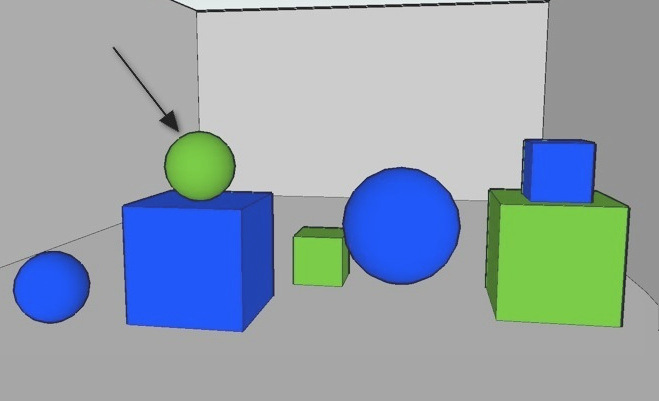
\includegraphics[width=.6\textwidth]{images/3.jpg}
\label{fig-GRE3D7}
\caption{Imagen del GRE3D7 corpus.}\label{contexto-evaluacion}
\end{figure}

La \textbf{exactitud}  es una m\'etrica autom\'atica estricta que se puede usar para comparar rankings de ERs. Es la proporci\'on de coincidencias perfectas entre la salida de algoritmo y las ERs generadas por humanos encontradas en corpora. 
La primer comparaci\'on de rankings de ERs se muestra en la Tabla \ref{results-algo-fig3}. Para cada ER, indicamos el n\'umero de veces que aparece en el corpus (\#Cor), la proporci\'on que representa (\%Cor), el n\'umero de veces que la gener\'o nuestro algoritmo (\#Alg) y la proporci\'on que representa (\%Alg).
Por \'ultimo, la exactitud (\%Acc) nos da el porcentaje de aciertos de las ERs generadas por el algoritmo y se calcula como el m\'inimo entre el \%Cor y \%Alg. 

\begin{table}[h]
\begin{small}
\begin{center}
\begin{tabular}{|l|r|r|r|r|r|}
\hline
\multirow{2}{*}{Expresiones Referenciales} & \multicolumn{2}{|c|}{Corpus} & \multicolumn{2}{|c|}{Algoritmo} & Exactitud \\ \cline{2-6} 
 & \#Cor & \multicolumn{1}{|c|}{\%Cor} & \multicolumn{1}{|c|}{\#Alg} & \multicolumn{1}{|c|}{\%Alg} & \multicolumn{1}{|c|}{\%Acc} \\
\hline
ball, green                                    & 91 & 65.00 & 6376 & 63.76 & 63.76 \\
ball, green, small                              & 23 & 16.43 & 3440 & 34.40 & 16.43 \\
ball, green, small, ontop(blue, cube, large)      &  8 &  5.71 &    0 &  0.00 &  0.00\\
ball, green, ontop(blue, cube)                  &  5 &  3.57 &    0 &  0.00 &  0.00\\
ball, green, ontop(blue, cube, large)            &  5 &  3.57 &    0 &  0.00 &  0.00\\
ball, green, small, ontop(blue, cube)            &  2 &  1.43 &    0 &  0.00 &  0.00\\
ball, ontop(cube)                             &  1 &  0.71 &   27 &  0.27 &  0.27 \\
ball, green, small, ontop(blue, cube, large, left) &  1 &  0.71 &    0 &  0.00 &  0.00\\
ball, small, ontop(cube,large)	              &  1 &  0.71 &    2 &  0.02 &  0.02 \\
ball, green, top                                &  1 &  0.71 &    0 &  0.00 &  0.00\\
ball, small, ontop(cube)                       &  1 &  0.71 &    3 &  0.03 &  0.03 \\
ball, green, ontop(cube)                       &  1 &  0.71 &    0 &  0.00 &  0.00\\
ball, front, green                              &  0 &  0.00 &   97 &  0.97 &  0.00\\
ball, front, green, small                        &  0 &  0.00 &   13 &  0.13 &  0.00\\
ball, front, top                                &  0 &  0.00 &   12 &  0.12 &  0.00\\
ball, green, left	                              &  0 &  0.00 &   11 &  0.11 &  0.00\\
ball, top                                      &  0 &  0.00 &   10 &  0.10 &  0.00\\
ball, green, left, small                         &  0 &  0.00 &    5 &  0.05 &  0.00\\
ball, left, top                                 &  0 &  0.00 &    2 &  0.02 &  0.00\\
ball, small, top                                &  0 &  0.00 &    1 &  0.01 &  0.00\\
ball, front, ontop(cube, left)                  &  0 &  0.00 &    1 &  0.01 &  0.00\\

\hline
Total & 140 & 100 & 10000 & 100 & 80.51 \\
\hline
\end{tabular}
\caption{ERs del corpus, y las producidas por nuestro algoritmo para la Figura~\protect\ref{contexto-evaluacion}.}\label{results-algo-fig3}
\vspace*{-.5cm}
\end{center}
\end{small}
\end{table}

 La exactitud del algoritmo con respecto al corpus GRE3D7 para esta escena es del 80\%. De las 14 ERs diferentes generadas por el algoritmo, 5 se encuentran en el corpus y las otras 9 no. Estas 9 expresiones referenciales incluyen propiedades de ubicaci\'on del target no con respecto a un landmark sino a su posici\'on en la escena 3D. Por ejemplo \emph{la esfera verde que est\'a a la izquierda} se refiere a que la esfera verde est\'a a la izquierda de la escena.  La probabilidad de uso de este tipo de propiedades es menor al 1\%, en particular la de left es 0,007, pero, como esa probabilidad no es cero, dichas propiedades aparecen en ERs (siempre con menos de un 1\% de frecuencia).  La m\'etrica de exactitud ha sido utilizada en trabajos anteriores para comparar la salida de un algoritmo de generaci\'on de ERs con las ERs que se encuentran en corpora~\cite{sluis07:eval,viet:gene11} y se considera una m\'etrica muy estricta para esta tarea.

\subsection{Evaluaci\'on autom\'atica sobre el corpus}
\label{sec:compara-varias}

Como es habitual cuando hacemos una evaluaci\'on con un caso particular, podemos pensar que como el algoritmo tiene un componente de azar, por eso nos dio bastante bien, para esa ejecuci\'on particular. Por eso aqu\'i se muestra la misma comparaci\'on realizada en la secci\'on anterior pero con todas las im\'agenes verde-azules del corpus GRE3D7. 
Para enriquecer esta parte mostraremos otros baselines, los cuales nos dar\'an pistas de que las probabilidades de uso aprendidas con el m\'etodo que presentamos en esta tesis son \'utiles para aproximar al ranking de ERs que aparece en corpora. Un baseline que se presenta ejecuta el algoritmo con una distribuci\'on aleatoria de probabilidades de uso. Llamamos uniforme a otro baseline, en el cual tomamos las ERs generadas por el sistema, las del corpus y las generadas con el modelo aleatorio les dimos la misma probabilidad de ocurrencia. Por ejemplo si eran 10 en total, y ejecutamos el algoritmo 100 veces, cada ER iba a aparecer 10 veces. En este baseline no ejecutamos el algoritmo. El Top baseline, es en el que el algoritmo us\'o las probabilidades de uso sacadas del corpus mismo. 

\bigskip

\begin{table}[h]
\begin{small}
\begin{center}
\begin{tabular}{|l|c|c|c|c|}
\hline
         &  \puse\ de escena & \puse\ aprendidas & \puse\ random & uniforme \\ \hline
Escena 1	&	85.75\%	&	84.49\%	&	17.95\%	&	5.37\%	\\
Escena 3	&	82.81\%	&	80.51\%	&	9.89\%	&	4.40\%	\\
Escena 6	&	90.11\%	&	83.30\%	&	4.13\%	&	4.16\%	\\
Escena 8	&	86.52\%	&	64.06\%	&	16.32\%	&	9.75\%	\\
Escena 10	&	89.49\%	&	75.80\%	&	7.56\%	&	3.70\%	\\
Escena 12	&	80.21\%	&	81.29\%	&	57.09\%	&	6.68\%	\\
Escena 13	&	89.98\%	&	50.79\%	&	9.30\%	&	3.59\%	\\
Escena 21	&	92.13\%	&	80.01\%	&	8.45\%	&	6.77\%	\\
\hline
Promedio	&	87.13\%	&	75.03\%	&	16.34\%	&	5.55\%	\\

\hline
\end{tabular}
\caption{exactitud entre las ERs del corpus y las generadas usando valores de \puse\ calculados desde la escena, aprendidos autom\'aticamente, provenientes de distribuciones random y uniforme.}\label{results-algo-all}
\end{center}
\end{small}
\end{table}


La primera columna muestra los valores obtenidos cuando corremos el algoritmo sobre la escena
con los valores de \puse\ obtenidos~\emph{de la propia escena}. Como se puede esperar,
esta columna tiene el mayor promedio de exactitud.

La segunda columna muestra los resultados del algoritmo cuando se ejecuta con \puse\ aprendido de
corpora como se explica en la Secci\'on~\ref{sec:learning} del cap\'itulo anterior. Este es el caso m\'as interesante porque muestra la capacidad de nuestra propuesta de generalizar a escenas no vistas con anterioridad y para las que no hay corpus. Para la mayor\'{i}a de las escenas la exactitud
es mayor al 80\% y la exactitud promedio es 75\%. La relativamente baja exactitud
obtenida en la escena 13 se explica principalmente por las pobres estimaciones del valor de~\puse\ para las palabras \emph{large} y \emph{small} que son propiedades vagas y no absolutas ya que dependen de cu\'an grandes son los objetos en relaci\'on con los otros elementos del contexto.  

En el corpus, las relaciones \emph{large} y \emph{small} se utilizan mucho m\'as cuando el target no puede ser identificado usando s\'olo propiedades taxon\'omicas (\emph{ball} y \emph{cube}) y propiedades absolutas (\emph{green} y \emph{blue}), pero las caracter\'{i}sticas que hemos utilizado para el aprendizaje autom\'atico no capturan dichas dependencias como se discute en la Secci\'on \ref{sec:learning-corpus} del Cap\'itulo \ref{sec:algoritmo}.
A pesar de esta limitaci\'on, el promedio de la segunda columna es 75\%. Para una m\'etrica como la de exactitud que es considerada demasiado estricta, estos resultados son buenos. Adem\'as, el 25\% no cubierto por el algoritmo puede contener ERs igualmente buenas como vamos a mostrar en la Secci\'on \ref{sec:humanevaluation}. Uno podr\'ia argumentar entonces que los valores de \puse\ aprendidos a partir del corpus son lo suficientemente buenos para ser utilizados para generar ERs para nuevas escenas del dominio.
Las dos \'ultimas columnas pueden ser consideradas como baselines. En la primera generamos
valores aleatorios para \puse\ y luego ejecutamos el algoritmo con esos valores de \puse.~La exactitud obtenida es en la mayor\'{i}a de los casos pobre, pero con
una variaci\'on notable debido al azar. Adem\'as estas ejecuciones toman mucho m\'as tiempo en finalizar, lo que indica que se est\'an realizando demasiadas particiones sin conseguir llegar a la meta. Esta observaci\'on de performance es consistente con los resultados de los experimentos de generaci\'on humana realizados por \cite{keysar:Curr98} y discutidos en la Secci\'on \ref{sec:psicolinguistica} del Cap\'itulo \ref{sec:seleccion}. Keysar argumenta que, las personas usan la prominencia de las propiedades en el dominio como heur\'istica para guiar la generaci\'on de ERs de forma de disminuir la carga cognitiva de tener que probar con todas las propiedades del dominio. Si la heur\'istica es buena, en muchos casos no es necesario ``revisar'' la ER para que identifique un\'ivocamente al target. Como efecto colateral de este proceso heur\'istico la ER resultante puede estar sobreespecificada, pero se genera r\'apidamente.  
Adem\'as de poca exactitud, cuando se utilizaron probabilidades random,  muchas de las ERs generadas suenan poco naturales y son dif\'iciles de realizar sin introducir ambig\"uedades como, por ejemplo, (\textit{peque\~na cosa sobre
el cubo azul que est\'a abajo de algo que es peque\~no}). En la \'ultima columna se presenta la exactitud de una corrida artificial, le llamamos uniforme, uniforme tomando todas las ERs de las dem\'as columnas y asign\'andoles la misma probabilidad. La uniforme consigue los peores resultados, ya que acumula ERs que no son del corpus, y las del corpus las tienen baja probabilidad. Para comparar nuestros resultados con los 3 baselines usamos tambi\'en la entrop\'ia cruzada.

En teor\'ia de la informaci\'on, la \textbf{entrop\'ia cruzada} entre dos distribuciones de probabilidad mide la media de bits necesarios para identificar un evento de un conjunto de posibilidades, si un esquema de codificaci\'on est\'a basado en una distribuci\'on de probabilidad dada q, m\'as que en la verdadera distribuci\'on p. Vamos a comparar la entrop\'ia cruzada entre la distribuci\'on de probabilidad que se encuentra en el corpus, y la distribuci\'on de ERs del corpus y las de ejecuciones del algoritmo con las probabilidades que acabamos de describir~(ver~\cite{juraksky:spee08} para obtener detalles sobre evaluaci\'on de entrop\'{i}a cruzada). En la Figura~\ref{Entrwopy} se muestran los resultados para las ocho escenas que hemos considerado.

Las entrop\'{i}as cruzadas de las dos primeras ejecuciones (\emph{escena} y \emph{aprendizaje autom\'atico}) son, en general, mucho m\'as cercanas de la entrop\'{i}a del corpus, que las entrop\'ias cruzadas de \emph{random} y \emph{uniforme}. S\'olo en la escena 12 random, por azar se acerca un poco m\'as.

\begin{figure}[h]
\centering
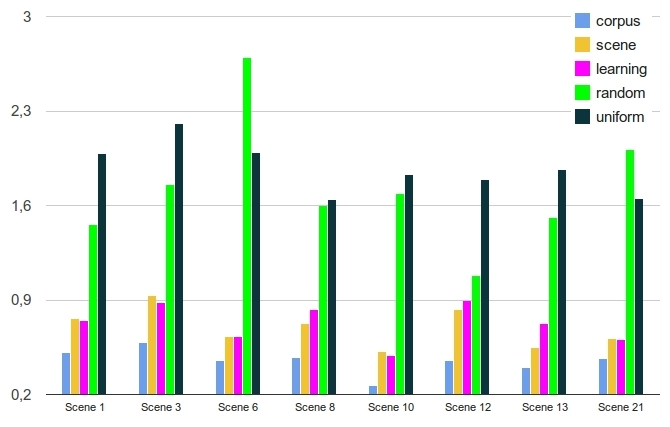
\includegraphics[width=0.8\textwidth]{images/entropy.jpg}
\caption{Entrop\'ia cruzada entre la distribuci\'on del corpus y diferentes baselines.}\label{Entropy}
\end{figure}
  
\bigskip
  

\section{Evaluaci\'on de rankings sobre el corpus TUNA} \label{sec:automaticevaluation}

En esta secci\'on se presenta la comparaci\'on de nuestro algoritmo con el algoritmo que tuvo el mejor desempe\~no en el TUNA Challenge. 

\subsection{El TUNA Challenge}
El TUNA Challenge, fue una serie de 2 desaf\'ios organizados en el 2008 y 2009 en el que se ped\'ia a los participantes desarrollar programas para generaci\'on de expresiones referenciales, donde pod\'ian generar s\'olo la selecci\'on de contenido o dar la realizaci\'on sint\'actica tambi\'en.
Se daba parte del corpus TUNA como entrenamiento, y un software de evaluaci\'on autom\'atica, el cual comparaba la salida del algoritmo con la ER humana del corpus TUNA. El algoritmo GRAPH fue el que mejores puntuaciones sac\'o en la competencia.
El algoritmo GRAPH que describimos en el Cap\'itulo \ref{sec:seleccion} es un algoritmo determin\'istico y por lo tanto produce la misma expresi\'on referencial cuando se ejecuta con el mismo target y contexto. Nuestro algoritmo es no-determin\'istico, puede dar una expresi\'on referencial diferente cada vez que se ejecuta. Con el fin de compararlos corremos nuestro algoritmo 100 veces y hacemos un ranking de las 20 ERs m\'as frecuentes generadas por el algoritmo. Utilizamos la parte de prueba del corpus TUNA (el cual fue introducido en la Secci\'on \ref{sec:corpusTUNA}), para comparar el ranking de ERs dado por nuestro algoritmo con las salidas del algoritmo GRAPH cuyos resultados se describen en~\cite{KrahmerGRAPH} y se reproducen en la Tabla~\ref{Tabla_sis_1_20}.


El algoritmo GRAPH define la generaci\'on de expresiones referenciales como un problema de b\'usqueda en un grafo, devuelve el grafo distintivo de menor costo (si existe) dada una funci\'on de costo particular. Comparamos a este algoritmo usando las m\'etricas exactitud, Dice y \textsc {masi}, introducidas en la Secci\'on \ref{sec:metricasAutomaticas}. 

Recordemos que el corpus TUNA tiene 2 partes, una parte cuyo dominio son muebles, y otra parte cuyo dominio son personas, ambos ubicados en una grilla. El corpus tiene una parte con target singular, y otra con targets plurales. Para realizar esta comparaci\'on se us\'o solamente la parte singular del corpus.


En la Tabla \ref{probability-of-use} y \ref{probability-of-use-people} se muestran las probabilidades de uso aprendidas desde el corpus. Se puede ver en la Tabla \ref{probability-of-use} por ejemplo que la probabilidad de usar {\it blue} es mucho m\'as alta que la probabilidad de usar {\it facing left} para describir al target. La probabilidad de usar {\it green} no es 0 porque se puede usar para describir a un landmark.

Para aprender las probabilidades de uso se sigui\'o el mecanismo descripto en el Cap\'itulo \ref{sec:algoritmo}, se unific\'o el vocabulario del corpus y se aprendi\'o una funci\'on de regresi\'on lineal por cada propiedad y se reemplazaron las variables por los valores correspondientes a cada escena. Se us\'o la parte de entrenamiento del corpus que consist\'ia del 80\% del corpus TUNA.

\bigskip

\begin{table}[H]
\begin{center}
\hspace*{.4cm}
 \begin{minipage}{0.48\textwidth} 
%\begin{center}
\begin{tabular}{|l|c|}
\hline
Relaciones Figura \ref{Tuna-scene} & \puse\ Aprendida \\
\hline
chair 	&	0.94	\\
blue 	&	0.89	\\
y3 	&	0.29	\\
x5 	&	0.27	\\
left 	&	0.25	\\
large 	&	0.21	\\
green 	&	0.05	\\
small 	&	0.05	\\
back 	&	0.02	\\
y1 	&	0.02	\\
\hline
\end{tabular}
%\hspace*{-.5cm}
\caption{Probabilidades aprendidas desde el corpus de la Figura~\ref{Tuna-scene}} 
\label{probability-of-use}

%\end{center}
\end{minipage}
\begin{minipage}{0.48\textwidth} 
%\begin{center}
\begin{tabular}{|l|c|}
\hline
Relaciones Figura \ref{Tuna-people-scene} & \puse\ Aprendida \\
\hline
person 	&	0.79	\\
hasGlasses 	&	0.71	\\
y2 	&	0.20	\\
x5 	&	0.18	\\
hasHair	&	0.13	\\
hairDark 	&	0.13	\\
hairLight 	&	0.11	\\
ageOld 	&	0.05	\\
y3 	&	0.03	\\
x2 	&	0.02	\\
\hline 
\end{tabular}
%\begin{center}
%\vspace*{.09cm}
\caption{Probabilidades de uso aprendidas desde el corpus para la Figura~\ref{Tuna-people-scene}} 
\label{probability-of-use-people}
%\end{center}
\end{minipage}
%\vspace*{-.9cm}
\end{center}
\end{table}

\begin{figure}[h]
\begin{subfigure}{.49\textwidth}
  \centering
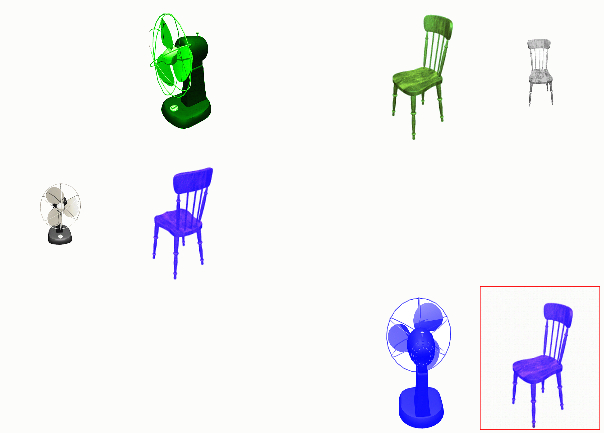
\includegraphics[width=\textwidth]{images/tuna.jpg}
\caption{El target de la escena es \emph{blue chair facing left}.}
\label{Tuna-scene}
\end{subfigure}
\begin{subfigure}{.49\textwidth}
 \centering
\vspace*{-.4cm}
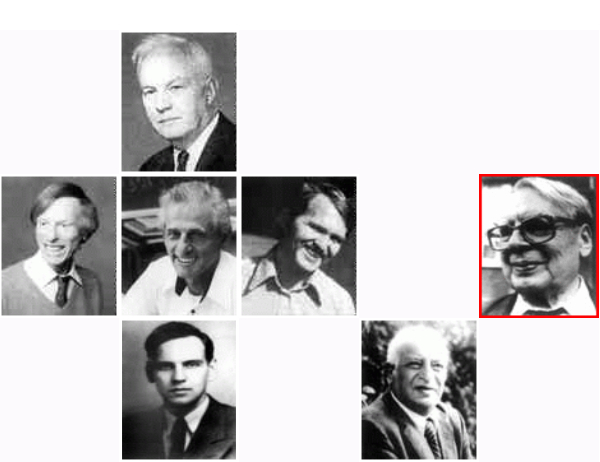
\includegraphics[width=\textwidth]{images/tuna-people.jpg}
\caption{El target de la escena es \emph{man with glasses}.} 
\label{Tuna-people-scene}
\end{subfigure}
\caption{Escenas usadas durante la recolecci\'on del corpus TUNA.} 
\end{figure}


%\vspace*{2cm}
%\begin{figure}[H]
%\centering
%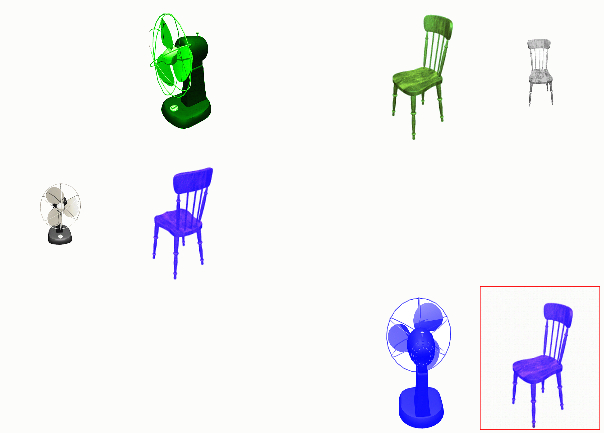
\includegraphics[width=0.5\textwidth]{images/tuna.jpg}
%%\vspace*{-.25cm}
%%\vspace*{-.4cm}
%\caption{Escena del TUNA corpus, el target \emph{blue chair facing left}.}
%\label{Tuna-scene}
%\end{figure}

%\begin{figure}[ht]
%%\begin{minipage}{0.60\linewidth}
%\centering
%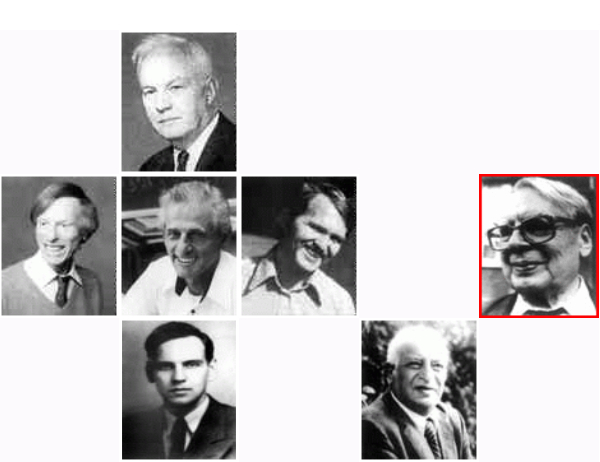
\includegraphics[width=0.5\textwidth]{images/tuna-people.jpg}
%%\vspace*{-.4cm}
%\caption{Escena usada durante la recolecci\'on del TUNA corpus. Para esta escena, la ER del target es \emph{the man with glasses}.} 
%\label{Tuna-people-scene}
%%\end{minipage}
%%\vspace*{-.38cm}
%%\begin{minipage}{0.50\linewidth}
%\centering
%%\vspace*{.2cm}
%%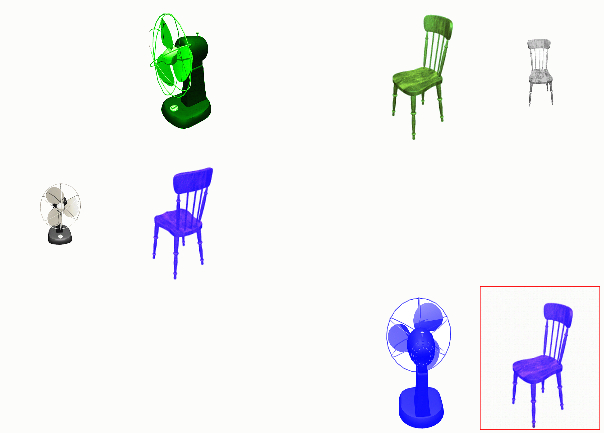
\includegraphics[width=\textwidth]{images/tuna.jpg}
%%\vspace*{-.25cm}
%%\vspace*{-.4cm}

%\caption{TUNA corpus furniture scene}
%\label{Tuna-furniture-scene}
%\end{minipage}
%\end{figure} 


Recordemos las m\'etricas autom\'aticas nombradas en la Secci\'on \ref{sec:metricasAutomaticas}, 
la \textbf{exactitud} se define como el porcentaje de coincidencias exactas entre cada ER producida por un ser humano y la producida por el sistema para la misma escena y target. Se considera que es una m\'etrica demasiado estricta. 
El coeficiente \textbf{Dice} es una m\'etrica de comparaci\'on de conjuntos al igual que \textbf{\textsc{masi}}, el valor va entre 0 y 1, 1 indica un matcheo perfecto entre los conjuntos. La diferencia entre ellas es que \textbf{\textsc{masi}} var\'ia en favor de la similaridad cuando un conjunto es un subconjunto de otro. Las dos son m\'etricas que no son tan estrictas como la exactitud por ejemplo con respecto al orden las palabras y justamente es lo que necesitamos ya que no estamos en la parte de realizaci\'on sint\'actica.

\begin{table}[h]
\begin{center}
\begin{tabular}{|l|c|c|c|}
\hline
	 	& 	Dice		&	\textsc{masi}	&	Exactitud		\\
\hline
sistema GRAPH, Dominio muebles	& 	80\% 		&	59\%	&	48\%		 	\\
sistema GRAPH, Dominio personas 	& 	72\%		&	48\%	&	28\%			\\
\hline
Nuestro sistema, Dominio muebles (top 1)	&	80\%		&	60\%	&	47\%		\\
Nuestro sistema, Dominio personas (top 1)	&	65\%		&	37\%	&	19\%		\\
\hline
Nuestro sistema, Dominio muebles (top 20)&	87\%		&	75\%  	&	65\%		\\
Nuestro sistema, Dominio personas (top 20)   &	81\%		&68\%	&	60\%		\\
\hline
\end{tabular}
%\vspace*{.1cm}
\caption{Comparaci\'on del algoritmo GRAPH y nuestro sistema. Consideramos 3 m\'etricas autom\'aticas para el top 1 y para el top 20 ERs producidas por nuestro algoritmo.}
%\vspace*{-.5cm}
\label{Tabla_sis_1_20}
\end{center}
\end{table}

En la Tabla~\ref{Tabla_sis_1_20} mostramos m\'etricas autom\'aticas y comparamos la performance de nuestro sistema con el sistema GRAPH para la primer ER del ranking (es decir, la m\'as frecuente) y para las primeras 20 ERs del ranking.
%\vspace*{-.5cm}
En la Figura~\ref{graficoPresicion} se muestra una comparaci\'on entre la exactitud de nuestro sistema y el sistema GRAPH. El gr\'afico de la izquierda corresponde al dominio muebles y el gr\'afico de la derecha corresponde al dominio personas. En el dominio muebles estamos obteniendo casi los mismos n\'umeros en las m\'etricas evaluadas.
Podemos ver que si tomamos la parte superior, es decir 1 ER (la primera, la m\'as probable), nuestra exactitud es menor que de GRAPH para el dominio de las personas. Sin embargo, si tenemos en cuenta las 20 mejores ERs que nuestro algoritmo es capaz de producir, podemos ver que la exactitud para ambos dominios se hace mayor del 60\% (60\% para personas y 65\% para muebles). Esto demuestra que nuestro algoritmo es capaz de generar ERs que son m\'as similares a las producidas por los seres humanos que el algoritmo GRAPH, aunque estas ERs no est\'en en primer lugar. Si el algoritmo GRAPH fuera modificado para ser no-determin\'istico es posible que tambi\'en mejorara su exactitud en 20 o m\'as ejecuciones. Esta es una l\'inea interesante de trabajo futuro. 

\begin{figure}[h]
\begin{subfigure}{.5\textwidth}
  \centering
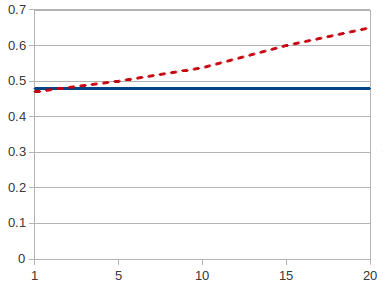
\includegraphics[width=\textwidth]{images/furniturePrec.png}
\caption{Muebles.}
\label{Tuna-scene-prec}

\end{subfigure}
\begin{subfigure}{.5\textwidth}
 \centering
  \centering
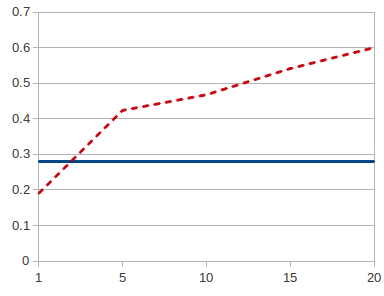
\includegraphics[width=\textwidth]{images/precP.png}
\caption{Personas.}
\end{subfigure}
\caption{Comparaci\'on de la exactitud  del algoritmo GRAPH y nuestro sistema. El eje x indica las x primeras ERs en el ranking. El eje y indica la exactitud. Nuestro sistema es representado como una l\'inea de puntos y GRAPH como una l\'inea continua.\label{graficoPresicion}}

\end{figure}

%\begin{figure}[H]
%\begin{subfigure}{.6\textwidth}
%  \centering
%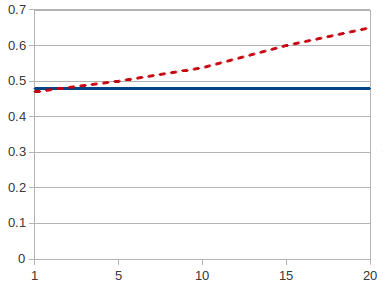
\includegraphics[width=\textwidth]{images/furniturePrec.png}
%\caption{}
%\end{subfigure}
%  \centering
%\begin{subfigure}{.6\textwidth}
%\centering
%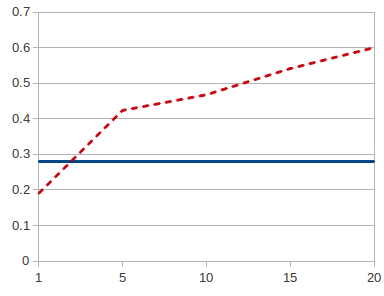
\includegraphics[width=\textwidth]{images/precP.png}
%\caption{}
%\end{subfigure}
%\caption{Comparaci\'on de la exactitud  del algoritmo GRAPH y nuestro sistema. El eje x indica que la exactitud se calcul\'o teniendo en cuenta las x primeras ERs en el ranking. El eje y indica la exactitud. Nuestro sistema es representado como una l\'inea de puntos y GRAPH como una l\'inea continua.\label{graficoPresicion}}
%\end{figure}

Otro resultado que podemos observar es que la exactitud  del top 1 en el dominio personas es mucho menor (19\%) que para el dominio de muebles (47\%), pero la exactitud se estabiliza cuando se consideran m\'as ERs de nuestro ranking. Esto puede explicarse por el hecho de que el conjunto del dominio de personas contiene muchas m\'as propiedades que se pueden elegir para describir a las personas que las que contiene el dominio de muebles.

Normalmente las m\'etricas autom\'aticas tienen la desventaja de calificar como malas a ERs que son buenas ERs, es decir identifican el target un\'ivocamente, en el contexto considerado, pero las consideran malas por no ser exactamente como las que aparecen en corpora. Otra manera de evaluar qu\'e tan buena es una ER es con evaluaciones manuales. Mostraremos una evaluaci\'on humana en la siguiente secci\'on.

%\newpage
 
\section{Evaluaci\'on humana} \label{sec:humanevaluation}

En las secciones anteriores describimos evaluaciones autom\'aticas de nuestro algoritmo. En esta secci\'on explicamos una evaluaci\'on humana que hicimos de las ERs generadas por nuestro algoritmo con las probabilidades de uso aprendidas para el TUNA corpus y descriptas en la secci\'on anterior.  

Como las ERs que generamos las generamos para el idioma ingl\'es, pedimos a dos jueces nativos de idioma ingl\'es evaluar nuestras expresiones referenciales a trav\'es de un experimento en la web. Los jueces podr\'{i}an entrar en el sistema de evaluaci\'on varias veces, es decir no ten\'ian que terminar la evaluaci\'on en la primera vez, para cada ER pod\'ian resolverla o pod\'ian volver a ella m\'as tarde. 

Durante la evaluaci\'on mostramos a cada juez una escena y dos ERs ordenadas al azar. Una ER correspond\'ia a la ER presente en el corpus TUNA producida por una persona para la escena y la otra ER correspond\'ia a la ER producida por nuestro sistema para la misma escena. Solicitamos a los jueces seleccionar la ER que ser\'{i}a m\'as \'util para identificar el target en la escena. El juez pod\'ia elegir una ER o indicar que las 2 ERs le parec\'ian igualmente buenas.

Nuestro objetivo es mostrar que incluso si la ER generada autom\'aticamente no coincide con la ER producida por un ser humano del corpus, puede ser juzgada como buena o incluso mejor que la ER generada por una persona.

En la Tabla~\ref{system-versus-human} se muestran los resultados del experimento de evaluaci\'on humana.
Las ERs producidas por el sistema en el top 1 fueron consideradas igual o mejor por los 2 jueces que las generadas por personas en el 75\% de los casos para los muebles y en el 43\% para las personas. Esto contrasta con el 47\% para muebles y 19\% para personas de la Tabla \ref{Tabla_sis_1_20}. Esto muestra que la m\'etrica de exactitud es demasiado estricta para la tarea, y las m\'etricas de DICE o \textsc {masi} se acercan m\'as a evaluaciones humanas. Adem\'as al menos 1 juez consider\'o que el 97\% de las ERs del sistema eran tan buenas o mejores que las humanas para los muebles y (87\% para las personas). Esto muestra que la evaluaci\'on de la calidad de las ERs es parcialmente subjetiva. S\'olo en el 8\% de los casos ambos jueces coincidieron que una ER generada autom\'aticamente era peor que la humana.

\begin{table}[H]
\begin{center}
\begin{tabular}{|l|c|c|c|}
\hline

 & Dominio muebles & Dominio personas & Media ponderada \\
\hline
sistema igual o mejor por 2 jueces  &.75  &       .43	&       .60 \\
sistema igual o mejor por 1 juez  &.97	&	.87	&	.92 \\
sistema peor por 2 jueces &	.03	&	.13	&	.08 \\
\hline
\end{tabular}
%\vspace*{.1cm}
\caption{Evaluaci\'on humana de las ERs del corpus con las generadas para escenas del corpus TUNA (parte singular).} 
\label{system-versus-human}
\vspace*{-.5cm}
\end{center}
\end{table}

A continuaci\'on, se ilustra el experimento de evaluaci\'on, mostrando ejemplos de casos en los que la expresi\'on del sistema fue considerada mejor por ambos jueces, por un solo juez o por ninguno de los dos.

Figura~\ref{smallBlueFan} ilustra un caso en el que el humano genera una ER subespecificada mientras que el sistema produce un ER que identifica de manera un\'{i}voca al target. La ER generada por el sistema para esta figura es {\it small blue fan}, mientras que la ER producida por el ser humano es {\it blue fan}. La ER del humano no logra identificar de forma \'unica el target y entonces no es preferida por los jueces humanos. Los seres humanos son conocidos por producir ERs subespecificadas, esto puede ser debido a las limitaciones cognitivas por no ser capaz de considerar todo el contexto referencial al mismo tiempo. Nuestro algoritmo es capaz de considerar todo el contexto referencial y combinar esta capacidad con la probabilidad de uso de las ERs aprendidas de los seres humanos.

\begin{figure}[H]
\begin{minipage}{0.48\linewidth}
\centering
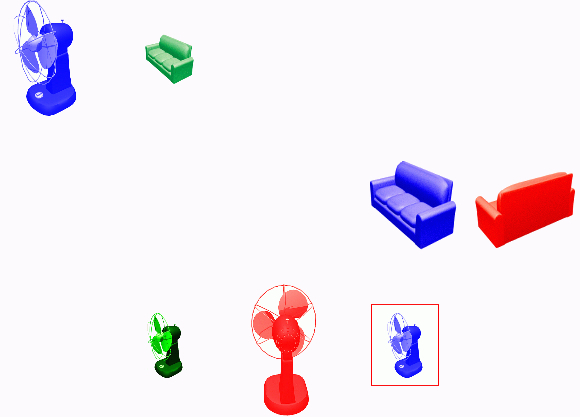
\includegraphics[width=\textwidth]{images/smallBlueFan.jpg}
\caption{Escena usada durante la recolecci\'on del TUNA corpus. La ER humana \emph{blue fan}, y la del sistema \emph{small blue fan}. Los jueces prefirieron la ER generada por el sistema.}
\label{smallBlueFan}
\end{minipage}
\hspace*{.04cm}
\begin{minipage}{0.48\linewidth}
\centering
\vspace*{.4cm}
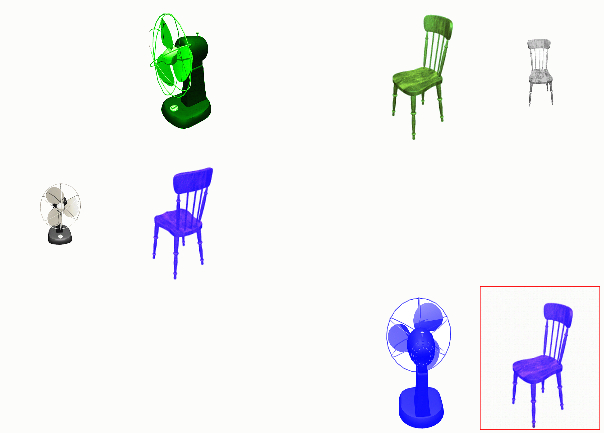
\includegraphics[width=\textwidth]{images/tuna.jpg} 
\vspace*{-.4cm}
\caption{Escena usada durante la recolecci\'on del TUNA corpus. La ER humana \emph{front blue chair}, y la del sistema \emph{bottom blue chair}. Ambos jueces humanos prefirieron la generada por el sistema.}
\label{BlueChair}
\end{minipage}
\end{figure}

En la Figura~\ref{BlueChair} la ER humana era {\it front blue chair}, y la ER sistema era {\it bottom blue chair}; ambos jueces seleccionaron la ER sistema. Este caso se puede explicar por el hecho de que, en este \'ambito, la propiedad {\it bottom} ayuda m\'as durante la identificaci\'on de la propiedad {\it front} porque concentra la atenci\'on del interlocutor en la parte inferior de la escena. Nuestro sistema aprende este hecho por el aprendizaje de un mayor valor de \puse\ para {\it bottom} que para {\it front} a partir de los datos de entrenamiento.

\begin{figure}[H]
\begin{minipage}{0.48\linewidth}
\centering
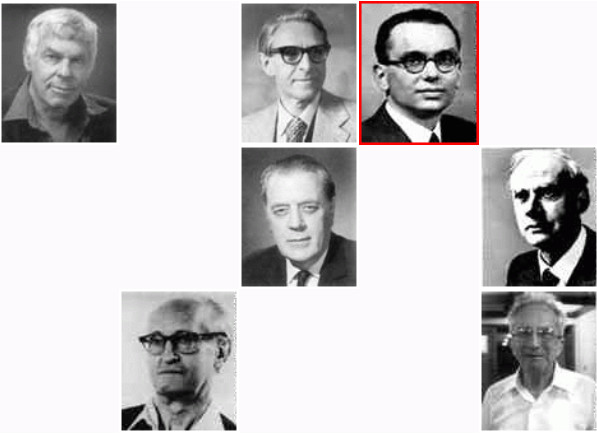
\includegraphics[width=\textwidth]{images/s59t26.jpg}
\caption{Escena usada durante la recolecci\'on del TUNA corpus. La ER humana \emph{the man with black hair}, y la del sistema \emph{the man wearing glasses in the fourth column}. Los jueces prefirieron la ER humana.}
\label{s28t25}
\end{minipage}
\hspace*{.04cm}
\begin{minipage}{0.48\linewidth}
\centering
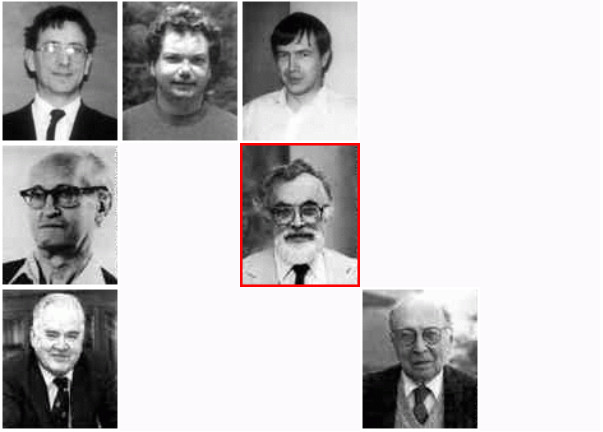
\includegraphics[width=\textwidth]{images/s315t21.jpg}
\vspace*{-.3cm}
\caption{Escena usada durante la recolecci\'on del TUNA corpus. La ER humana \emph{man with a beard},  y la del sistema \emph{man with a beard wearing glasses}. Los jueces no estuvieron de acuerdo en su preferencia.}
\label{s307t21}
\end{minipage}
\end{figure}

Figura~\ref{s28t25} es un ejemplo en el que ambos jueces prefirieron la expresi\'on humana. La ER humana era {\it the man with black hair}, y del sistema de {\it the man wearing glasses in the fourth column}. Este ejemplo pone de manifiesto el hecho de que, en el dominio de las personas algunas propiedades son m\'as destacadas en algunas im\'agenes que en otros debido a diferentes tonos de colores. Propiedades graduables como estas (en contraste con las propiedades absolutas) son todav\'{i}a un problema abierto para los algoritmos de GER.

Figura~\ref{s307t21}~ilustra un caso en el que la ER del sistema era m\'as sobreespecificada que la ER humana; el sistema incluye {\it wearing glasses}, mientras que el ser humano no lo hizo. En este caso un sujeto humano prefiere la ER del sistema y el otro la ER del humano. La cantidad de sobreespecificaci\'on es una cuesti\'on subjetiva, donde los humanos mismos no est\'an de acuerdo. Una evaluaci\'on donde las ERs se utilicen para resolver una tarea ser\'{i}a interesante para investigar este asunto.

\section{Notas finales y linkeo del cap\'itulo}\label{sec:notas5}

En este cap\'itulo se present\'o una evaluaci\'on autom\'atica de los rankings de ERs generados por el algoritmo sobre 2 benchmarks del \'area, uno el corpus GRE3D7 y otro son los resultados de una competencia el TUNA challenge, en este caso nos comparamos con el algoritmo que mejores puntuaciones tuvo en la competencia. Presentamos tambi\'en una evaluaci\'on humana sobre ERs del corpus TUNA y las generadas por el algoritmo. Si bien conseguimos buenas puntuaciones en el siguiente cap\'itulo veremos una evaluaci\'on de un caso mucho m\'as natural, en el que consideramos ERs generadas por el algoritmo para puntos de inter\'es en mapas. 
